
%(BEGIN_QUESTION)
% Copyright 2009, Tony R. Kuphaldt, released under the Creative Commons Attribution License (v 1.0)
% This means you may do almost anything with this work of mine, so long as you give me proper credit

This PLC is being used to start and stop an electric motor, and also to shut it down automatically if any of three ``shutdown'' conditions occur:

\begin{itemize}
\item{} Excessive vibration
\item{} Overcurrent (overload heater contact)
\item{} High winding temperature
\end{itemize}

$$\includegraphics[width=15.5cm]{i04426x01.eps}$$

$$\includegraphics[width=15.5cm]{i04426x02.eps}$$

An instrument technician is asked to physically remove the temperature switch from service in order to perform a routine calibration check on it, while bypassing the automated PLC shutdown system so that the motor will still run while the temperature switch is pulled out of service.  The technician decides she will jumper terminal {\tt X4} on the PLC's input card to terminal {\tt L1} on the power supply card in preparation to remove the switch.  Do you agree that this is the proper step to take before removing the switch?  If not, propose an alternative course of action.

\underbar{file i04426}
%(END_QUESTION)





%(BEGIN_ANSWER)

If the technician jumpers input {\tt X4} to {\tt L1}, the motor will immediately shut down.  What should be done is to {\it disconnect} the temperature switch from input {\tt X4}.

%(END_ANSWER)







%(BEGIN_NOTES)

{\bf This question is intended for exams only and not worksheets!}.

%(END_NOTES)


